% might need psfig, url, amsmath, amsfonts?
\documentclass[psfig]{acm_proc_article-sp}

\begin{document}

\title{StreaMIT: A Language for Streaming Applications\thanks{This
document is {\bf MIT/LCS Technical Memo LCS-TM-620}, August 2001.  A similar
version was submitted to POPL 2002.  Please do not distribute.}}

\numberofauthors{1}
\author{
\alignauthor \vspace{-18pt} Bill Thies, Michal Karczmarek, and Saman Amarasinghe\\
	\vspace{12pt}
	Laboratory for Computer Science \\
	Massachusetts Institute of Technology \\
	Cambridge, MA  02139 \\
	\vspace{12pt}
	{\tt \{thies, karczma, saman\}@lcs.mit.edu} \\
	\vspace{12pt}
	\mbox{August 13, 2001}
}

% for the arrow of a function def, etc.
\newcommand{\ma}[2]{max_{#1 \rightarrow #2}}
\newcommand{\mal}[1]{maxloop_{#1 \rightarrow #1}}
\newcommand{\mi}[2]{min_{#1 \leftarrow #2}}

\maketitle

\begin{abstract}
As DSP programming is becoming more complex, there is an increasing
need for high-level abstractions that can be efficiently compiled.
Toward this end, we present a set of aggressive optimizations that
target linear sections of a stream program.  Our input language is
StreamIt, which represents programs as a hierarchical graph of
autonomous filters.  A filter is linear if each of its outputs can be
represented as an affine combination of its inputs.  Linear filters
are common in DSP applications; examples include FIR filters,
expanders, compressors, FFTs and DCTs.

We present a linear extraction analysis that automatically detects
linear filters based on the C-like code in their {\tt work} function.
Once linear filters are identified, we show how neighboring nodes can
be collapsed into a single linear representation, thereby eliminating
many redundant computations.  Also, we describe a method for
automatically translating linear nodes into the frequency domain,
thereby yielding algorithmic savings for convolutional filters.

We have completed a fully-automatic implementation of the above
techniques as part of the StreamIt compiler, and we demonstrate
performance improvements that average 400\% over our benchmark
applications.




\end{abstract}

\section{Introduction}

Applications that are structured around some notion of a ``stream''
are becoming increasingly important and widespread.  There is evidence
that streaming media applications are already consuming most of the
cycles on consumer machines \cite{Rix98}, and their use is continuing
to grow.  In the embedded domain, applications for hand-held
computers, cell phones, and DSP's are centered around a stream of
voice or video data.  The stream abstraction is also fundamental to
high-performance applications such as intelligent software routers,
cell phone base stations, and HDTV editing consoles.

Despite the prevalence of these applications, there is surprisingly
little language and compiler support for practical, large-scale stream
programming.  Of course, the notion of a stream as a programming
abstraction has been around for decades \cite{SICP}, and a number of
special-purpose stream languages have been designed (see
\cite{survey97} for a review).  Many of these languages and
representations are elegant and theoretically sound, but they often
lack features and are too inflexible to support straightforward
development of modern stream applications, or their implementations
are too inefficient to use in practice.  Consequently, most
programmers turn to general-purpose languages such as C or C++ to
implement stream programs.

There are two reasons that general-purpose languages are inadequate for
stream programming.  Firstly, they are a mismatch for the application
domain.  That is, they do not provide a natural or intuitive
representation of streams, thereby having a negative effect on
readability, robustness, and programmer productivity.  Moreover, because
the widespread parallelism and regular communication patterns of data
streams are left implicit in general-purpose languages, compilers are
not stream-conscious and do not perform stream-specific optimizations.
As a result, performance-critical loops are often hand-coded in a
low-level assembly language and must be re-implemented for each target
architecture.  This practice is labor-intensive, error-prone, and very
costly.

Secondly, general-purpose languages are a mismatch for the emerging
class of grid-based architectures \cite{smartmemories,rawshort,trips} that
are especially well-suited for stream processing.  Perhaps the primary
appeal of C is that it provides a ``common machine language'' for
von-Neumann architectures.  That is, it abstracts away the
idiosyncratic differences between machines, but encapsulates their
common properties: a single program counter, arithmetic operations,
and a monolithic memory.  However, for grid-based architectures, the
von-Neumann model no longer holds, as there are multiple instruction
streams and distributed memory banks.  Thus, C no longer serves as a
common machine language--in fact, it provides the wrong abstraction
for the underlying hardware, and architecture-specific directives are
often needed to obtain reasonable performance.  Again, this greatly
complicates the job of the programmer and hampers portability.

StreamIt is a language and compiler specifically designed for modern
stream programming.  The StreamIt language has two goals: first, to
provide high-level stream abstractions that improve programmer
productivity and program robustness within the streaming domain, and
second, to serve as a common machine language for grid-based
processors.  At the same time, the StreamIt compiler aims to perform
stream-specific optimizations to achieve the performance of an expert
programmer.

This paper motivates, describes, and justifies the high-level language
features of StreamIt, version 1.0.  The major limitation of StreamIt
1.0 is that all flow rates in the streams must be static; applications
such as compression that have dynamically varying flow rates will be
the subject of future work.  A large set of applications can be
implemented with static rates, and while dynamic rates will require a
different runtime model, it will still be essential to fully analyse
and optimize static sub-sections in order to obtain high performance.

The paper is organized as follows. In Section {\ref{sec:domain}}, we
characterize the domain of streaming programs that motivates the
design of StreamIt, and in Section~\ref{sec:overview} we describe the
language features in detail.  We present an in-depth example of a
software radio in Section~\ref{sec:example}, preliminary results in
Section~\ref{sec:results}, related work in Section~\ref{sec:related},
and conclusions in Section~\ref{sec:conc}.


\section{Streaming Application Domain}
\label{sec:domain}

The applications that make use of a stream abstraction are diverse,
with targets ranging from embedded devices, to consumer desktops, to
high-performance servers.  Examples include systems such as the Click
modular router \cite{click} and the Spectrumware software radio
\cite{spectrumware,softwareradio}; specifications such as the
Bluetooth communications protocol \cite{bluetooth}, the GSM Vocoder
\cite{gsm}, and the AMPS cellular base station\cite{amps}; and almost
any application developed with Microsoft's DirectShow library
\cite{directshow}, Real Network's RealSDK \cite{realsdk} or Lincoln
Lab's Polymorphous Computing Architecture \cite{pca}.

We have identified a number of properties that are common to such
applications--enough so as to characterize them as belonging to a
distinct class of programs, which we will refer to as {\it streaming
applications.}  We believe that the salient characteristics of a
streaming application are as follows:

\begin{enumerate}
\item {\it Large streams of data.}  Perhaps the most fundamental
aspect of a streaming application is that it operates on a large (or
virtually infinite) sequence of data items, hereafter referred to as a
{\it data stream}.  Data streams generally enter the program from some
external source, and each data item is processed for a limited time
before being discarded.  This is in contrast to scientific codes,
which manipulate a fixed input set with a large degree of data reuse.

\begin{figure*}[t]
\centering
\vspace{-6pt}
\psfig{figure=Radio.eps,width=4.75in}
\vspace{-10pt}
\caption{A block diagram of our frequency-hopping software radio.}
\vspace{-6pt}
\label{fig:radiodiagram}
\end{figure*}

\item {\it Independent stream filters.}  Conceptually, a streaming computation
represents a sequence of transformations on the data streams in the
program.  We will refer to the basic unit of this transformation as a
{\it filter}: an operation that--on each execution step--reads one or
more items from an input stream, performs some computation, and writes
one or more items to an output stream.  Filters are generally
independent and self-contained, without references to global variables
or other filters.  A stream program is the composition of filters into
a {\it stream graph}, in which the outputs of some filters are
connected to the inputs of others.

\item {\it A stable computation pattern.}  The structure of the stream
graph is generally constant during the steady-state operation of a
stream program.  That is, a certain set of filters are repeatedly
applied in a regular, predictable order to produce an output stream
that is a given function of the input stream.

\item {\it Occasional modification of stream structure.}  Even though
each arrangement of filters is executed for a long time, there are
still dynamic modifications to the stream graph that occur on
occasion.  For instance, if a wireless network interface is
experiencing high noise on an input channel, it might react by adding
some filters to clean up the signal; a software radio re-initializes a
portion of the stream graph when a user switches from AM to FM.
Sometimes, these re-initializations are synchronized with some data in
the stream--for instance, when a network protocol changes from
Bluetooth to 802.11 at a certain point of a transmission.  There is
typically an enumerable number of configurations that the stream graph
can adopt in any one program, such that all of the possible
arrangements of filters are known at compile time.

\item {\it Occasional out-of-stream communication.}  In addition to
the high-volume data streams passing from one filter to another,
filters also communicate small amounts of control information on an
infrequent and irregular basis.  Examples include changing the volume
on a cell phone, printing an error message to a screen, or changing a
coefficient in an upstream FIR filter.

\item {\it High performance expectations.}  Often there are real-time
constraints that must be satisfied by streaming applications; thus,
efficiency (in terms of both latency and throughput) is of primary
concern.  Additionally, many embedded applications are intended for
mobile environments where power consumption, memory requirements, and
code size are also important.
\end{enumerate}





 






\section{StreamIt Overview}

Most data-flow or signal-processing algorithms can be broken down into
a number of simple blocks with connections between them.  In StreamIt
parlance, the smallest block is a \emph{filter}; it has a single input
and a single output, and its body consists of Java-like code.  Filters
are then connected by placing them into one of three composite blocks:
pipelines, split-joins, and feedback loops.  Each of these structures
also has a single input and a single output, so these blocks can be
recursively composed.

A typical streaming application might be a software FM radio, as shown
in Figure \ref{fig:fm-radio}.  The program receives its input from an
antenna, and its output is connected to a speaker.  The main program
is a pipeline with a band-pass filter for the desired frequency, a
demodulator, and an equalizer; the equalizer in turn is made up of a
split-join, where each child adjusts the gain over a particular
frequency range, followed by a filter that adds together the outputs
of each of the bands.

\begin{figure}[htbp]
  \begin{center}
    \includegraphics{cookbook.0}
    \caption{Stream graph for a software FM radio}
    \label{fig:fm-radio}
  \end{center}
\end{figure}

Our goal with choosing these constructs was to create a language with
most of the expressiveness of a general data-flow graph structure, but
to keep the block-level abstraction that modern programming languages
offer.  Allowing arbitrary graphs makes scheduling and partitioning
difficult for the compiler.  The hierarchical graph structure allows
the implementation of blocks to be ``hidden'' from users of the block;
for example, an FFT could be implemented as a single filter or as
multiple filters, but so long as there is a stream structure named
``FFT'' somewhere in the program the actual implementation is
irrelevant to other modules that use it.  Since most graphs can be
readily transformed into StreamIt structures, StreamIt is suitable for
working on a wide range of signal-processing applications.

%%% Local Variables:
%%% TeX-master: "cookbook.tex"
%%% End:

\section{Semantics of Time}
\label{sec:time}
In this section we develop a more formal semantics for the message
delivery guarantees described above.  The timing model in StreamIt is
unique in that all time is relative to {\it information
wavefronts}--that is, two independent filters can describe a common
time only in terms of when the {\it effects} of one filter's execution
are seen by the other.  Thus, although each filter's {\tt work}
function is invoked asynchronously without any notion of global time,
two invocations of a work function occur at the same
``information-relative time'' if they operate on the same information
wavefront.

To define this notion more precisely, we present transfer functions
that describe the flow of information across filters and streams.
Using these transfer functions, we translate message delivery
constraints into a set of constraints on the execution schedule of the
stream graph.  Finally, we use these scheduling constraints to
formulate an operational semantics for messaging and latency in
StreamIt.

\subsection{Information Flow}

The concept of information flow is central to the streaming domain.
When an item enters a stream, it carries with it some new information.
As execution progresses, this information cascades through the stream,
effecting the state of filters and the values of new data items which
are produced.  We refer to an ``information wavefront'' as the
sequence of filter executions that first sees the effects of a given
input item.  This wavefront is well-defined even in the presence of
rate-changing filters that peek or pop a different number of items
than they push.
\begin{figure}
\centering
\psfig{figure=Tapes.eps,width=3.2in}
\caption{A filter's input and output tapes during an execution step.  With each step, the filter pushes two items, pops two items, and peeks at three additional items.  The initial state of the input tape is shown at left.  The center shows the filter with both input and output tapes during the invocation of {\tt work}.  The final state of the output tape is shown at right}
\label{fig:tapes}
\end{figure}
To formalize the wavefront, we introduce some new representations for
the state of the stream graph.  Consider that in place of each data
channel there is an infinite ``tape'' which contains the history of
values that have been pushed onto the channel (see Figure
\ref{fig:tapes}).  Now consider the following functions:
\begin{itemize}
\item Given that there are $x$ items on tape $a$, the maximum number
of items that can appear on tape $b$ is $\ma{a}{b}(x)$.

\item Given that there are $x$ items on tape $b$, the minimum number
of items that must appear on tape $a$ is $\mi{a}{b}(x)$.
\end{itemize}
Note that these functions are only defined over pairs of tapes $(a,
b)$ where $a$ is {\it upstream} of $b$--that is, where there is a
directed path in the stream graph from the filter following $a$ to the
filter preceding $b$.  We will say that the filter $b$ is {\it
downstream} of $a$ under exactly these same conditions.

The $max$ and $min$ functions are related to the information wavefront
in the following sense.  The item at position $y = \mi{a}{b}(x)$ of
tape $a$ is the latest item on tape $a$ to {\it affect} the item at
position $x$ of tape $b$.  This is because item $x$ on tape $b$ can be
produced if and only if tape $a$ contains at least $y$ items.  Note
that this effect might be via a control dependence rather than a data
dependence--for instance, if item $y$ needed to pass through a
round-robin joiner before some data from another stream could be
routed to tape $b$.  However, when speaking of the information
wavefront, we only consider information passed through the data
streams; if a data item affects another via a low-latency downstream
message, then this effect could jump ahead of the wavefront.

We now turn to deriving expressions for $\ma{a}{b}$ and $\mi{a}{b}$.
Doing so will allow us to formalize the semantics of messaging and
latency in StreamIt, as well as enabling static verification
techniques such as deadlock and overflow detection.

\subsubsection{Filters}

Consider a filter $A$ that peeks $peek_A$, pops $pop_A$, and pushes
$push_A$ data items on every execution step.  Further, let us denote
the input and output tapes of $A$ by $I_A$ and $O_A$, respectively.
We now turn our attention to finding $\ma{I_A}{O_A}$ and
$\mi{I_A}{O_A}$, describing the transfer of information across the
filter $A$.

\begin{figure}
\centering
\psfig{figure=pipeline.eps,width=2.0in}
\caption{\protect\small Stream construct with labeling.
\protect\label{fig:pipelinelabel}}
\end{figure}

To derive $\ma{I_A}{O_A}(x)$, observe that the filter can execute so
long as it does not peek beyond the $x$'th item on the input tape,
$I_A$.  After the $n$'th execution, it has popped $n*pop_A$ items,
peeked up to $n*pop_A + (peek_A - pop_A)$, and pushed $n*push_A$
items.  Thus, it can execute $n = \lfloor(x - (peek_A - pop_A)) /
pop_A)\rfloor$ times, leaving the following expression for
$\ma{I_A}{O_A}(x)$:
\[
\begin{array}{l}
\ma{I_A}{O_A}(x) = \\ \\
\makebox[.1in]{ } \left\{
\begin{array}{ccl}
push_A*\left\lfloor\frac{x-(peek_A-pop_A)}{pop_A}\right\rfloor & if & x \ge (peek_A-pop_A) \\
 & \\
0 & if & x < (peek_A-pop_A) \\
\end{array} \right.
\end{array}
\]
By identical reasoning, the reader can verify the following
expression for $\mi{I_A}{O_A}(x)$:
\begin{align*}
\mi{I_A}{O_A}(x) = \left\lceil\frac{x}{push_A}\right\rceil*pop_A+(peek_A-pop_A)
\end{align*}
\subsubsection{Pipelines}

Let us now derive expressions for $min$ and $max$ in the case of
pipelined filters.  In the base case, consider that two filters are
connected, with the output of $A$ feeding into the input of $B$ (see
Figure~\ref{fig:pipelinelabel}).  We are seeking $\ma{I_A}{O_B}(x)$:
the maximum number of items that can appear on tape $O_B$ given that
there are $x$ items on tape $I_A$.  Observing that a maximum of
$\ma{I_A}{O_A}(x)$ items can appear on tape $O_A$, and that $O_A$ must
equal $I_B$ since the filters are connected, we see that a maximum of
$\ma{I_B}{O_B}(\ma{I_A}{O_A}(x))$ items can appear on $O_B$:
\begin{align*}
\ma{I_A}{O_B} = \ma{I_B}{O_B} \circ \ma{I_A}{O_A}
\end{align*}
In the case of $\mi{I_A}{O_B}(x)$, the order of composition is
reversed: given that there are $x$ items on tape $O_B$, a minimum of
$\mi{I_B}{O_B}(x)$ are on tape $I_B$, and since $O_B = I_A$, we have
that a minimum of $\mi{I_A}{O_A}(\mi{I_B}{O_B}(x))$ items appear on
$I_A$, leaving:
\begin{align*}
\mi{I_A}{O_B} = \mi{I_A}{O_A} \circ \mi{I_B}{O_B}
\end{align*}
By identical reasoning, these composition laws hold for pipelined
streams as well as filters.  That is, given tapes $x$, $y$, and $z$, 
we have that:
\begin{align}
\label{eq:compose}
\begin{split}
\ma{x}{z} &= \ma{y}{z} \circ \ma{x}{y} \\
\mi{x}{z} &= \mi{x}{y} \circ \mi{y}{z}
\end{split}
\end{align}
However, there are some restrictions on these definitions.  They only
apply when there is a downstream path $P_1$ from the filter following
$x$ to the filter preceding $y$, a downstream path $P_2$ from the
filter following $y$ to the filter preceding $z$, and the paths $P_1$
and $P_2$ are non-overlapping.  This restriction prevents the
successive composition of transfer functions around feedback loops,
thereby ensuring a unique definition for all pairs $(x, z)$ where
there is a downstream path from $x$ to $z$.

\subsubsection{SplitJoins}

\begin{figure}
\centering
\psfig{figure=splitjoin.eps,width=3.2in}
\caption{\protect\small SplitJoin construct with labeling.
\protect\label{splitjoin}}
\end{figure}

We now derive $min$ and $max$ in the case of a SplitJoin, as pictured
in Figure \ref{splitjoin}.  For the splitter $S$ there are two output
tapes; let us denote them by $O1_S$ and $O2_S$.  Similarly, let us
denote the two input tapes of the joiner $J$ by $I1_J$ and $I2_J$.  We
derive below the transfer functions the round robin and
duplicate/combine nodes.  Note that the duplicate/combine nodes can be
simulated with round robins and duplicating filters, but we provide
the transfer functions anyways to simplify the semantic analysis of a
program.  We have yet to derive these expressions for the weighted
round robin nodes.

{\bf Round robin splitter.}  In the case of a round-robin splitter, the
items from the input tape are alternately routed to the output tapes,
with the first item going onto tape $O1_S$.  By this definition, we
can see that the splitter's $max$ is defined as follows:
\begin{align*}
\ma{I_S}{O1_S}(x) &= \left\lceil\frac{x}{2}\right\rceil \\
\ma{I_S}{O2_S}(x) &= \left\lfloor\frac{x}{2}\right\rfloor
\end{align*}
To derive the $min$ function across a splitter, observe that the input
tape need only progress so far as to produce the items on the emptier
output tape.  That is, we need to consider the number of items on both
of the splitter's output to determine the minimum number of items that
are needed at its input.  Thus, our $min$ function has two arguments:
the first corresponding to $O1_S$ and the second corresponding to
$O2_S$.  The equation is as follows:
\begin{align*}
\mi{I_S}{(O1_S, O2_S)}(x_1, x_2) = MIN(2*x_1-1, 2*x_2)
\end{align*}
{\bf Round robin joiner.}  The rules for a round robin joiner are in
some sense dual to those of the round robin splitter.  Again assuming
that items are alternately drawn from the input tapes, starting with
$I1_J$, we have that:
\begin{align*}
\mi{I1_J}{O_J}(x) &= \left\lceil\frac{x}{2}\right\rceil \\
\mi{I2_J}{O_J}(x) &= \left\lfloor\frac{x}{2}\right\rfloor
\end{align*}
Again, the $max$ function takes two arguments, corresponding to the
number of items on $I1_J$ and $I2_J$, respectively:
\begin{align*}
\ma{(I1_J, I2_J)}{O_J}(x_1, x_2) = MIN(2*x_1-1, 2*x_2)
\end{align*}
{\bf Duplicate splitter}.  Clearly, the $max$ function of a duplicate
splitter is simply the identity function, since it maps each element
on the input tape to the same location on the output tapes:
\begin{align*}
\ma{I_S}{O1_S}(x) &= x \\
\ma{I_S}{O2_S}(x) &= x
\end{align*}
The $min$ function is similar, except that--like the round robin
split--the input need only progress as far as the lesser output:
\begin{align*}
\mi{I_S}{(O1_S, O2_S)}(x_1, x_2) = MIN(x_1, x_2)
\end{align*}
{\bf Combine joiner.} The combine joiner is simply the dual of the
duplicate splitter, with transfer functions that the reader can verify
as follows:
\begin{align*}
\ma{(I1_J, I2_J)}{O_J}(x_1, x_2) &= MIN(x_1, x_2) \\
\mi{I1_J}{O_J}(x) &= x \\
\mi{I2_J}{O_J}(x) &= x
\end{align*}

\subsubsection{FeedbackLoops}

\begin{figure}
\centering
\psfig{figure=feedback.eps,width=3.2in}
\caption{\protect\small  FeedbackLoop construct with labeling.
\protect\label{looplabel}}
\end{figure}

We have to be careful when defining the transfer functions for
feedback loops (see Figure \ref{looplabel}).  The feedback splitter
$FS$ serves as a normal splitter, and has the same $min$ and $max$
functions as defined above.  However, the feedback joiner $FJ$ is
slightly different than a standard joiner, since during the first few
executions it fabricates values from the loop body before they appear
on the input tape.  The transfer function must take special account of
these initial values, since they never appear on $I2_{FJ}$, the input
tape from the loop body.  This is because we model the initialization
of FeedbackLoops by feeding the joiner the initial values directly
instead of pushing them onto a channel.

Let $n$ be the number of initial values that are provided to the
feedback joiner before values from the feedback loop are read.  Let
$J$ be a normal COMBINE or ROUND\_ROBIN joiner as defined for
SplitJoins.  Now, let us define the transfer functions for $FJ$, the
feedback joiner.

The $min$ function for the main stream is as before:
\begin{align*}
\mi{I1_{FJ}}{O_{FJ}} = \mi{I1_J}{O_J} 
\end{align*}
However, we must offset by $n$ when considering the $min$ function
that draws from the loop's tape:
\begin{align*}
\mi{I2_{FJ}}{O_{FJ}}(x) = \mi{I2_J}{O_J}(x) - n
\end{align*}
Finally, the $max$ function must be similarly shifted for the input
from the loop:
\begin{align*}
\ma{(I1_{FJ}, I2_{FJ})}{O_{FJ}}(x_1, x_2) = \ma{(I1_J, I2_J)}{O_J}(x_1,
x_2 + n)
\end{align*}

\subsubsection{Summary}

We have derived expressions for $\ma{a}{b}$ and $\mi{a}{b}$ for when
$a$ and $b$ are the respective input and output to 1) a filter, 2) a
pipeline, 3) a split or join, and 4) a feedback split or join.  By
composing these expressions following Equation~\ref{eq:compose}, we
can arrive at values of $\ma{a}{b}$ and $\mi{a}{b}$ for all pairs of
tapes $(a, b)$ where there is some directed path through the stream
graph--that is, along the direction of data flow--from the filter
reading from tape $a$ to the filter writing to tape $b$.  

Ommitted from the above analysis are: 1) weighted round robin nodes,
2) filters that push or pop items from within their {\tt init}
functions, and 3) message handlers that send messages themselves.  We
hope to address these issues in a future document.

\subsection{Semantics}

Equipped with definitions of $\ma{a}{b}$ and $\mi{a}{b}$, we can now
address the semantics of StreamIt's message delivery and latency
guarantees.

\subsubsection{Messages}

Suppose that filter $A$ sends a message to filter $B$ with latency
$\lambda$, where $\lambda$ is any integer.  In $\lambda$ invocations
of $A$'s {\tt work} function, $A$ will produce one or more data items
$d$.  Now, the messaging system guarantees that:
\begin{enumerate}
\item If $B$ is upstream of $A$, then $B$ will receive the message
immediately following the last invocation of its {\tt work} function
which produces items that affect $d$.

\item If $B$ is downstream of $A$, then $B$ will receive the message
immediately preceding the first invocation of its {\tt work} function
which produces items that are effected by $d$.

\item If $B$ runs in parallel with $A$, then the message timing is in terms
of a shared set of splitters and joiners.  We are developing semantics
for this case, but they are beyond the scope of this paper.
\end{enumerate}
These guarantees can be expressed more formally as a set of
constraints on the number of items on certain tapes in the system.  We
will use $n(t)$ to represent the number of items on tape $t$ at a
given point of execution.  Again, suppose that filter $A$ sends a
message to filter $B$ with latency $\lambda$, where $\lambda$ is any
integer.  Let $s$ be equal to $n(O_A)$ at the time that the message
was sent.  We have that:

\begin{enumerate}

\item If $B$ is upstream of $A$, the message will be delivered when:
\begin{align}
\label{eq:msgup}
n(O_B) = \mi{O_B}{O_A}(s + push_A * \lambda)
\end{align}
That is, $s + push_A * \lambda$ is the number of items on $A$'s output tape
after producing the data of interest.  Then, $y =
\mi{O_B}{O_A}(s + push_A * \lambda)$ is the latest item on $B$'s output
tape that affects the data of interest.  The message should be
delivered immediately after the work function producing this item,
which occurs when the item count $n(O_B)$ equals $y$, as specified by
the constraint.

\item If $B$ is downstream of $A$, the message will be delivered when:
\begin{align}
\label{eq:msgdown}
n(O_B) = \ma{O_A}{O_B}(s + push_A * (\lambda-1))
\end{align}
That is, $s + push_A * (\lambda - 1)$ is the number of items on $A$'s
output tape before pushing the data of interest, and $y =
\ma{O_A}{O_B}(s + push_A * (\lambda-1))$ is the maximum number of items
on $B$'s output tape as a result of the outputs of $A$.  Thus, when
$A$ pushes the next set of data, it could affect the data that will be
pushed next onto the output tape of $B$.  (Note that the next set of
data from $A$ might not be sufficient to calculate the next set on
$B$'s output, but it could affect it nonetheless.)  The message must
be delivered immediately before this effected data appears on $B$'s
output, so the number of items $n(O_B)$ on $B$'s output must equal $y$.

\end{enumerate}

\subsubsection{Latency}

Each directive {\tt MAX\_LATENCY(A, B, n)} has the same effect as
defining a message from filter $B$ to upstream filter $A$ with latency
$n$.

\subsubsection{Scheduling}

We can fully define the possible sequences of filter executions as a
set of constraints on the number of items on each tape in the stream
graph.  This is useful not only from the perspective of semantics, but
for compiler analysis of the space of valid schedules.  To begin the
analysis, we formulate the constraints imposed by message delivery
guarantees on the number of items on each tape.

Suppose that a filter $A$ might send a message to filter $B$ with a
maximum latency of $\lambda$ during any invocation of its work
function.  Then we must constrain the execution of $B$ to make sure
that it is not too far ahead to receive the message with the given
latency.  That is, we can only execute $B$ so long as $n(O_B)$--the
item count on its output tape--does not exceed the count when a
message would be delivered.  Recalling the expression for message
delivery time (Equations \ref{eq:msgup} and
\ref{eq:msgdown}), this constraint is as follows if $B$ is upstream of $A$:
\begin{align}
\label{eq:mc1}
n(O_B) \le \mi{O_B}{O_A}(n(O_A) + push_A * \lambda)
\end{align}
and as follows if $B$ is downstream of $A$:
\begin{align}
\label{eq:mc2}
n(O_B) \le \ma{O_A}{O_B}(n(O_A) + push_A * (\lambda-1))
\end{align}
The guarantees for latency are treated identically to message
guarantees, as fitting with the semantics of latency as described
above.

{\bf Defining the schedule.}  We now have a set of constraints
expressing whether or not a given set of tapes respects the latency
and message delivery guarantees in a program.  We will now
incorporate these constraints into an operational semantics that
defines a legal sequences of filter executions.  

We represent a stream graph as a configuration $(\langle p(t_1),
n(t_1) \rangle,$ $\langle p(t_2), n(t_2) \rangle,$ $\dots,$ $\langle
p(t_k), n(t_k) \rangle)$, where $p(t)$ represents the number of items
that have been popped from tape $t$, and $t_1
\dots t_k$ are the tapes in the stream graph.  Obviously, we have the
constraint that $p(t) \le n(t)$ for each tape $t$, since a filter can
only pop as many items as have appeared on its input tape.

When the program begins, no items have been pushed or popped from any
data channels.  Thus, each tape is empty, and the starting
configuration $C_0$ is simply the zero vector.  It is possible that
the initial configuration violates some of the constraints imposed by
the messaging and latency constructs, in which case the compiler can
inform the programmer that the delivery constraints requested in the
program are unsatisfiable.

Let ${\cal P}(C)$ denote whether or not the constraints in
Equations~\ref{eq:mc1} and~\ref{eq:mc2} are satisfied for all filters
in a stream graph with configuration $C$.  We can then write the
transition function between configurations as follows:
\[
\begin{scriptsize}
\begin{array}{c}
n(I_A) - p(I_A) \ge peek_A; \\ (\dots , \langle p(I_A), n(I_A) \rangle, \dots,
\langle p(O_A), n(O_A) \rangle, \dots); \\ {\cal P}((\dots , \langle p(I_A)+pop_A, n(I_A) \rangle, \dots,
\langle p(O_A), n(O_A)+push_A \rangle, \dots)); \\ \hline (\dots , \langle p(I_A)+pop_A,
n(I_A) \rangle, \dots, \langle p(O_A), n(O_A)+push_A \rangle, \dots)
\end{array}
\end{scriptsize}
\]
There are two components of this rule.  On the first line, we state
that, for filter $A$ to fire, there must be at least $peek_A$ items on
$A$'s input tape that have not yet been popped.  Secondly, we express
that once $A$ has fired, the new configuration must satisfy the
messaging and latency constraints ${\cal P}$.  The new configuration differs
from the original only in that $pop_A$ items have been popped from
$A$'s input and $push_A$ items have been pushed to $A$'s output.

{\bf Bounding the buffer size.}  It is a straightforward extension to
incorporate a constraint on the maximum number of live items in the
stream.  This could be useful both from a language perspective, in
which a user might wish to constrain the buffer size, or from a
compiler perspective, in which the scheduler is interested in
constraining the number of live items.

The live items in a given configuration are those that have been
pushed to a channel but have not yet been popped.  That is, the buffer
size needed for a configuration $(\langle p(t_1), n(t_1) \rangle,$
$\dots,$ $\langle p(t_k), n(t_k) \rangle)$ is $\sum_{i=0}^k n(t_i) -
p(t_i)$.  If we wish to bound the number of live items to MAXITEMS,
then, we need only add one condition to the transition rule:
\[
\begin{scriptsize}
\begin{array}{c}
n(I_A) - p(I_A) \ge peek_A; \\ (\dots , \langle p(I_A), n(I_A) \rangle, \dots,
\langle p(O_A), n(O_A) \rangle, \dots); \\ {\cal P}((\dots , \langle p(I_A)+pop_A, n(I_A) \rangle, \dots,
\langle p(O_A), n(O_A)+push_A \rangle, \dots)); \\ \sum_{i=0}^k n(t_i) - p(t_i) \le
MAXITEMS; \\ \hline (\dots , \langle p(I_A)+pop_A, n(I_A) \rangle, \dots, \langle p(O_A),
n(O_A)+push_A \rangle, \dots)
\end{array}
\end{scriptsize}
\]

\subsection{Program Verification}

A number of program analysis techniques are also enabled by the $min$
and $max$ functions that we have defined.  In particular, it is very
simple to compute 1) whether or not the program will deadlock as a
result of a starved input channel, and 2) whether or not any buffer
will grow without bound during the steady-state execution of the
program.

{\bf Deadlock detection.}  The deadlock detection algorithm takes
advantage of the fact that the only loops in our stream graph are part
of a FeedbackLoop construct.  A stream graph will be deadlock-free if
and only if there is no net change of output rate in the feedback
loop.  This can be formulated in terms of the $max$ function by
requiring that the wavefront from the output of the feedback joiner
$FJ$ unto itself is the identity function.  However, since we were
careful to leave the $max$ function undefined over cycles in the
stream graph, we define a new function $maxloop$ that maps a given
feedback joiner to the information wavefront around the loop:
\begin{align*}
\mal{FJ}(x) \equiv \ma{I2_FJ}{O_FJ} \circ \ma{O_FJ}{I2_FJ}
\end{align*}
The order of composition is as in Equation \ref{eq:compose} for the
composition of pipelines. Also, for the purposes of calculating
$\mal{FJ}$, one must assume that there are an infinite number of items
on tape $I1_{FJ}$; that is, the join from the feedback loop is not
limited by the external data source.

Finally, we can state the constraint that the feedback loop must
respect.  For a loop with declared latency $\lambda$, the loop will neither
overflow nor deadlock if:
\begin{align*}
\mal{FJ}(x) = x + \lambda
\end{align*}
If $\mal{FJ}(x)$ is less than $x + \lambda$, then there will be deadlock in
the program.

{\bf Overflow detection.}  There are two places that a buffer can
overflow in the stream graph.  The first is in a feedback loop, when
$\mal{FJ}(x)$ (calculated above) is more than $x + \lambda$.  The second
case is when the parallel streams of a split/join have different
production rates.  For a splitter $S$ and a joiner $J$, the production
rates will cause an overflow if and only if $\ma{O1_S}{I1_J}(x) -
\ma{O2_S}{I2_J}(x)$ is not $O(1)$.  This difference could be analyzed
by a compiler for every SplitJoin in the stream graph to verify that
no buffers will overflow during steady-state execution.

\begin{figure}[t]
\centering
\psfig{figure=fir-block.eps,width=3.2in}
\caption{A block diagram of a five tap FIR filter.}
\label{fig:firfilter}
\end{figure}




\section{MSL Use-Case Examples}

As an example, we will illustrate the commands required to set up and
run a filter on a single core. For simplicity, we assume the filter is
connected to a buffer that provides a FIFO abstraction over tapes (the
input buffer is the input tape, and the output buffer is the output
tape). The filter has a single input tape, single output tape, and
static rates: its work function pops $i$, peeks $i+e$, and pushes $o$
bytes per iteration.

Before the filter can be run, it must be loaded, its input and output
buffers must allocated, and the filter's tapes must be attached to the
buffers. The commands that perform this are illustrated in
Figure~\ref{fig:lib:init}.

\begin{figure}[!htb]
\begin{center}
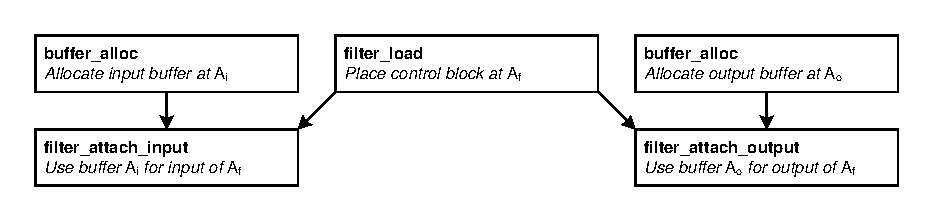
\includegraphics[scale=.55]{figs/init}
\end{center}
\caption[Commands to set up a filter.]{Commands to load a filter and allocate and attach input and output buffers. Lines between commands represent dependencies that must be specified to the library when the commands are issued. These commands may be issued in one or multiple groups.}
\label{fig:lib:init}
\end{figure}

In addition, input data must be transferred into the input buffer before the filter can be run, and output data must eventually be transferred out of the output buffer. With an initially empty input buffer, the commands to transfer in $n$ iterations of input, run the filter for $n$ iterations, and then transfer out $n$ iterations of output (assuming that the input and output buffers were sized appropriately) are shown in Figure~\ref{fig:lib:run}.

\begin{figure}[!htb]
\begin{center}
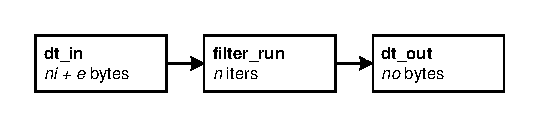
\includegraphics{figs/run}
\end{center}
\caption[Commands to run a filter.]{Commands to run a filter for the
  first $n$ iterations, including transferring input and output. The
  corresponding data transfer commands on other cores are not shown.}
\label{fig:lib:run}
\end{figure}

A sequence of commands is required to run the filter for a larger
number of iterations on a core with a finite local store
capacity. This is illustrated in Figure~\ref{fig:lib:ext}.

\begin{figure}[!htb]
\begin{center}
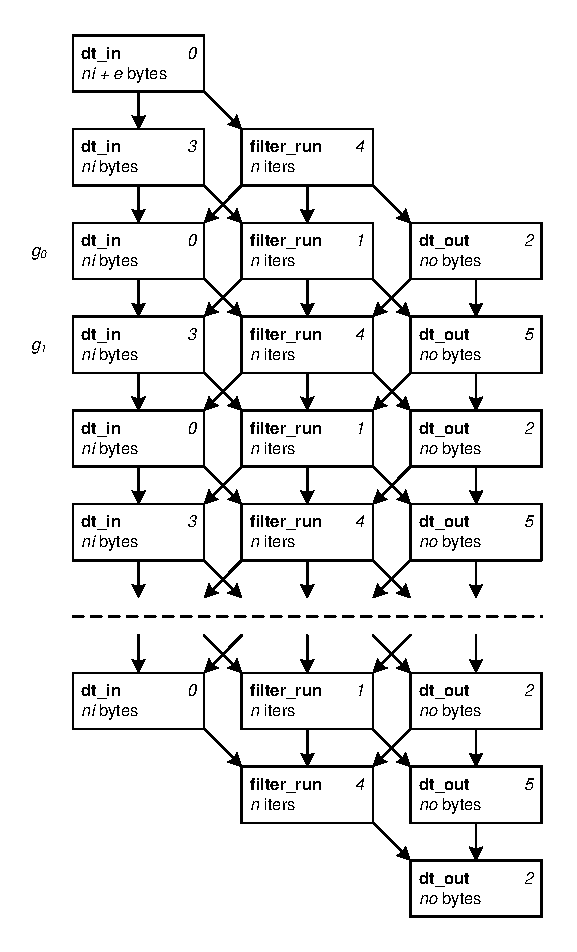
\includegraphics[scale=.90]{figs/ext}
\end{center}
\caption[Sequence of commands to run a filter for a large number of iterations.]{Sequence of commands to run a filter for a large number of iterations. Command IDs are indicated in the upper right. Each row is issued as a different group.}
\label{fig:lib:ext}
\end{figure}

Provided that the input buffer is at least $2ni+e$ bytes and the output buffer is at least $2no$ bytes, the dependencies among the commands in the sequence ensure that:
\begin{itemize}
\item When a \textsf{dt\_in} command becomes active, there are at most $ni+e$ bytes of data in the input buffer, and thus enough space to transfer in an additional $ni$ bytes.
\item When a \textsf{dt\_out} command becomes active, there are at least $no$ bytes of data in the output buffer, and thus enough data to transfer out.
\item When a \textsf{filter\_run} command becomes active, there are at least $ni+e$ bytes of data in the input buffer and at most $no$ bytes of data in the output buffer. This is enough input data and output space to run the filter for $n$ iterations.
\end{itemize}

This sequence of commands effectively ``pipelines'' the basic operation from Figure~\ref{fig:lib:run}. Double-buffering is accomplished when the data transfer commands in a group complete before the \textsf{filter\_run} does. In this case, the following \textsf{filter\_run} has no outstanding dependencies once the current \textsf{filter\_run} completes, and can become active immediately.

The user or scheduler can keep the core continually supplied with work
by initially issuing the first two groups, thereafter issuing the next
group whenever a group completes. In this case, the core almost always
has two groups of commands issued, with one group active and the other
queued. In addition, with the exception of the first two and last two
groups, the command parameters, IDs and dependencies in every other
group are identical. This allows the user to initially set up two
groups ($g_0$ and $g_1$ in Figure~\ref{fig:lib:ext}) and repeatedly
issue them for a majority of the execution. If executions are
relatively long, the overhead of the first and last group, where no
filter is being run, will be amortized effectively. Alternatively, the
user can load another filter and run it during those gaps.

In practice, situations such as the above, where a static-rate filter
is run for a large number of iterations and large amounts of input and
output data are transferred, are very common in streaming code. To
avoid requiring the user to manually issue groups and deal with
command completion callbacks in every such case, the MSL library also
provides extended operations that encapsulate this pattern. In an
extended operation, the user provides the library with filter rates,
the addresses of opposing buffers on other processors for data
transfers, and the number of groups to run for; the library issues and
responds to all commands internally and notifies the user when the
entire operation is complete.
%% Where one or both opposing buffers are located in memory,
%% the library also handles the PPE side of data transfers
%% internally. 
Extended operations greatly simplify setting up pipelines
of any length where all filters in the pipeline have static rates.


\section{Related Work}
\label{sec:related}

Software pipelining for clustered vliws \cite{qian02}.

The Imagine stream processor~\cite{rixner98bandwidthefficient}
supports a time-multiplexed execution model.  The architecture
contains 48 parallel ALU's organized into 6 VLIW clusters.  The
programming model requires the programmer to write computation filters
in Kernel-C and stitch them together using Stream-C.  Because the
execution unit is data-parallel, the compiler uses time multiplexing
to execute a single filter at a time across all of the parallel
clusters.  While this provides perfect load balancing and high
arithmetic utilization when there is abundant data parallelism, it
suffers when a filter has retained state or data-dependences between
iterations.  Moreover, architectures based solely on
time-multiplexing do not scale spatially, as there are global wires
orchestrating the parallel execution units. 

Previous work in compiling StreamIt to Raw has taken a purely space
multiplexed approach~\cite{streamit-asplos}.  In this model, a single
filter was mapped to each execution tile.  To support applications
with more filters than execution tiles, a partitioning algorithm was
employed to adjust the granularity of the graph by fusing adjacent
filters into one.

Previous work in scheduling computation graphs to parallel targets
have focused on dynamic techniques \cite{SDFSched, SDFSched2,
may87communicating, DAGSched}. In general, multiple graph nodes are
{\it clustered} onto a single computational node and scheduled
dynamically.  

Our work, unlike most previous work in this field,
models link contention and topography.  Furthermore, StreamIt graphs
are implicitly formed of loops so we can apply loop scheduling
techniques such as software pipelining to build our schedules.

%The problem of instruction scheduling for MIMD and VLIW architectures
%is similar to the problem tackled by the space-time compiler.  ILP
%compilers for clustered VLIW architectures~\cite{Bulldog, Multiflow}
%are decomposed into stages that are analogous to the stages of the
%SpaceTime compiler.  These compilers must partition or cluster
%instructions, assign instructions to processors, and then schedule the
%instructions.  

Previous work on software pipelining has focused on scheduling machine
instructions in a loop \cite{lam-softpipe, rau-softpipe} to a
uniprocessor target.  The algorithms devised must account for tight
resource constraints and complex instruction dependences.  Our
software-pipelining problem is much less constrained, a traditional
modulo scheduling algorithm can not effectively take advantage of this
flexibility.  Previous work on ILP scheduling for the Raw
architectures ~\cite{lee98spacetime} also bears similarity.  However,
these compilers schedule graphs of fine-grained instructions. The
partitioning and scheduling heuristics are mindful of a different set
of constraints including different types of dynamism and less regular
communication patterns as compared to StreamIt graphs.

As far as we know, we are the first to apply loop-level scheduling
techniques to the problem of scheduling coarse-grained task graphs.

% \cite{cheops-thesis}
%   http://web.media.mit.edu/~kung/publication/thesis.pdf
%
% other possible things to cite:
%  http://portal.acm.org/citation.cfm?id=801721&dl=ACM&coll=portal
%  http://www.csrl.unt.edu/~kavi/Research/ica3pp156.pdf
%  http://cdmetcalf.home.comcast.net/papers/cop/node1.html#SECTION00010000000000000000

\section{Conclusions and Future Work}
\label{sec:conclusion}

This paper makes two contributions.  First, it introduces teleport
messaging: a powerful language construct enabling precise message
delivery between nodes of a distributed stream program.  In comparison
with other methods to implement messaging functionality in a
Synchronous Dataflow (SDF) model, teleport messaging is arguably more
readable, more robust, and easier to maintain.  In addition, our
implementation of teleport messaging in the StreamIt compiler resulted
in a 49\% performance improvement for a frequency hopping radio
running on a cluster of workstations.  Like several declarative
language constructs, teleport messaging improves performance by
exposing the true dependences to the compiler and allowing it to
optimize the communication.

%% We outlined several possible applications of $\sdep$, including
%% latency constraints, debugging, speculation, and program analysis, and
%% we look forward to pursuing these directions in the future.

Second, this paper formulates $\sdep$, a natural and useful dependence
representation for the streaming domain.  While this paper applies
$\sdep$ to a new language construct, we envision other applications as
well.  For example, $\sdep$ could be used in a debugger to identify
which iterations of an upstream actor are affecting a given iteration
of a downstream actor.  In a software-based speculation
system~\cite{frank-thesis}, $\sdep$ could be applied to trace the
effects of a failed prediction and to roll back the appropriate actor
executions.  $\sdep$ also offers a new method for measuring latency in
a stream graph.  Similar to representations such as dependence
levels~~\cite{AK82}, direction vectors~\cite{wolfe82}, and dependence
polyhedra~\cite{Irig88} for scientific programs, $\sdep$ provides
dependence information that could be used to test or verify program
transformations.

There are some limitations in the current study that are fertile
grounds for future research.  First, our formulation of $\sdep$
requires a directed path in the stream graph (aligned with the
direction of data flow) between the actors in question.  We are
generalizing $\sdep$ to actors that run in parallel by leveraging
their data dependences with common predecessors (upstream) or
successors (downstream).  Second, as detailed in
Section~\ref{sec:constraints}, we do not solve the general scheduling
problem that incorporates overlapping constraints from teleport
messaging; even determining whether or not a set of constraints is
feasible (especially during the initialization
schedule~\cite{karczma-thesis}) seems to be an interesting question.
Third, in the current model only actors can send and receive messages.
We are extending this into a hierarchical model where stream
containers (such as pipelines) can also receive events and dispatch
them precisely to other streams.  Finally, our approach relies on the
static communication rates present in SDF.  It would be interesting to
consider teleport messaging in a more dynamic context; for example,
downstream non-negative latency messages could be immediately
supported by embedding messages in data items, while other messages
might require speculative delivery or modified timing contracts.

Our work can be viewed as the integration of dynamic behavior into a
static dataflow language.  Our insight is that there is a class of
control messages that only adjust a parameter in the target actor;
they do not otherwise affect the input or output channels upon
delivery.  This model enables a hybrid scheduling scheme in which the
steady-state dataflow is exactly orchestrated at compile time, but
there are windows in which a message could adjust an internal field of
an actor between its execution steps.  We consider this to be a
promising avenue for creating a unified development environment that
captures all aspects of stream application development without
sacrificing either performance or programmability.

\bibliographystyle{abbrv}
\bibliography{references,elliotw,thies}
\begin{figure*}
\centering
\psfig{figure=fft-pre-tape.eps,width=4.8in}
\caption{The bit reverse order filter in the FFT, with N=8. The tapes illustrate the data re-shuffling.}
\label{fig:bitreverseorder}
\end{figure*}

\begin{figure*}
\centering
\psfig{figure=fft-butterfly-tape.eps,width=5.8in}
\caption{The 4x4 butterfly stage in the FFT. The tapes illustrates the data transformation and computation.}
\label{fig:butterfly}
\end{figure*}

\begin{figure}
\vspace{-0.6in}
\scriptsize
\begin{verbatim}
class RFtoIF extends Filter {
   Channel input = new FloatChannel();
   Channel output = new FloatChannel();
   int size, count;
   float weight[];
   void init(float f) {
      setf(f);
   }
   void work() {
      output.push(input.pop()*weight[i++]);
      if (count==size) count = 0;
   }
   void setf(float f) {
      count = 0;
      size = CARRIER_FREQ/f*N;
      weight = new float[size];
      for (int i=0; i<size; i++)
         weight[i] = sine(i*PI/size);
   }
}

class FIR extends Filter {
   Channel input = new FloatChannel();
   Channel output = new FloatChannel();           
   int N;
   void init(int N) {
      this.N = N;
   }
   void work() {
      float sum = 0;
      for (int i=0; i<N; i++) {
         sum += input.peek(i)*FIR_COEFF[i][N];
      }
      input.pop();
      output.push(sum);
   }
}

class Booster extends Stream {
   void init(int N, boolean adds) {
      if (adds) add(new FIR(N));
   }
}

class Butterfly extends Stream {
   void init(int N, int W) {
      add(new SplitJoin() {
         void init() {
            setSplitter(WEIGHTED_ROUND_ROBIN(N, N));
            add(new Filter() {
               Channel input = new FloatChannel();
               Channel output = new FloatChannel();
               float weights[] = new float[W];
               int curr;
               void init() {
                  for (int i=0; i<W; i++)
                     weights[i] = calcWeight(i, N, W);
                  curr = 0;
               }
               void work() {
                  output.push(input.pop()*weights[curr++]);
                  if(curr>= W) curr = 0;
               }    
            });
            add(IDENTITY());
            setJoiner(ROUND_ROBIN);
      }});
      add(new SplitJoin() {
         void init() {
            setSplitter(DUPLICATE);
            add(new Filter() {   
               Channel input = new FloatChannel();
               Channel output = new FloatChannel();
               void work() {
                  output.push(input.pop() - input.pop());
               }
            });
            add(new Filter() {   
               Channel input = new FloatChannel();
               Channel output = new FloatChannel();
               void work() {
                  output.push(input.pop() + input.pop());
               }
            });
            setJoiner(WEIGHTED_ROUND_ROBIN(N, N));
      }});
}}
\end{verbatim}
\vspace{-6pt}
\caption{\protect\small A Trunked Radio Receiver in StreaMIT.
\protect\label{fig:radiocode}}
\vspace{-12pt}
\end{figure}

\begin{figure}
\vspace{-0.6in}
\scriptsize
\begin{verbatim}
class FFT extends Stream {
   void init(int N) {
      add(new SplitJoin() {
         void init() {
            setSplitter(WEIGHTED_ROUND_ROBIN(N/2, N/2));
            for (int i=0; i<2; i++) 
               add(new SplitJoin() {
                  void init() {
                     setSplitter(ROUND_ROBIN);
                     add(IDENTITY());
                     add(IDENTITY());
                     setJoiner(WEIGHTED_ROUND_ROBIN(N/4, N/4));
               }});
            setJoiner(ROUND_ROBIN);
      }});
      for (int i=2; i<N; i*=2)
        add(new Butterfly(i, N));
}}

class CheckFreqHop extends SplitJoin {
   RFtoIFPortal freqHop;
   void init(RFtoIFPortal freqHop) {
      this.freqHop = freqHop;
      setSplitter(WEIGHTED_ROUND_ROBIN(N/4-2,1,1,N/2,1,1,N/4-2));
      int k = 0;
      for (int i=1; i<=5; i++) {
         if ((i==2)||(i==4)) {
            for (int j=0; j<2; j++) {
               add(new Filter() {
                  Channel input = new FloatChannel();
                  Channel output = new FloatChannel();
                  void work() {
                     float val = input.pop();
                     if (val >= MIN_THRESHOLD) 
                        freqHop.setf(FREQ[k], new TimeInterval(4*N, 6*N)); 
                     output.push(val);
                  }
               });
               k++;
            }
         } else add(IDENTITY());
      }
      setJoiner(WEIGHTED_ROUND_ROBIN(N/4-2,1,1,N/2,1,1,N/4-2));
   }
}

class CheckQuality extends Filter {
   Channel input = new FloatChannel();
   Channel output = new FloatChannel();
   float aveHi, aveLo;
   BoosterPortal boosterSwitch;
   boolean boosterOn;
   void init(BoosterPortal boosterSwitch, boolean boosterOn) {
      aveHi = 0; aveLo = 1;
      this.boosterSwitch = boosterSwitch;
      this.boosterOn = boosterOn;
   }
   void work() {
      float val = input.pop();
      aveHi = max(0.9*aveHi, val);
      aveLo = min(1.1*aveLo, val);
      if (aveHi - aveLo < QUAL_BAD_THRESHOLD && !booosterOn) {
         boosterSwitch.init(true, BEST_EFFORT);
         boosterOn = true;
      }
      if(aveHi - aveLo > QUAL_GOOD_THRESHOLD & boosterOn) {
         boosterSwitch.init(false, BEST_EFFORT);
         boosterOn = false;
      }
      output.push(val);
   }
}

class TrunkedRadio extends Stream {
   int N = 64;
   RFtoIFPortal freqHop = new RFtoIFPortal();
   BoosterPortal onOff = new BoosterPortal().
   void init() {
      ReadFromAtoD in = add(new ReadFromAtoD());
      RFtoIF rf2if = add(new RFtoIF(STARTFREQ));
      Booster iss = add(new Booster(N, false));
      add(new FFT(N));
      add(new CheckFreqHop(freqHop));
      add(new CheckQuality(onOff, false));
      AudioBackEnd out = add(new AudioBackEnd());

      freqHop.register(rf2if);
      onOff.register(iss);
      MAX_LATENCY(in, out, 10);
   }
}
\end{verbatim}
\vspace{-12pt}
\end{figure}


%\vspace{.5in}
\newpage

\newcommand{\doc}[1]{{\bf {\tt #1}} \vspace{3pt} \\}

\renewcommand{\theequation}{A-\arabic{equation}}
% redefine the command that creates the equation no.
\setcounter{equation}{0}  % reset counter 
\setcounter{section}{0}

\begin{center}
\large{\bf{APPENDIX:  Details on Java Syntax \vspace{6pt} \\ ***DRAFT***}}
\end{center}

\section{Java Classes}

A diagram of the Java class hierarchy for StreaMIT is shown in
Figure~\ref{fig:hierarchy}.  A summary of the methods in each class is
as follows.

\subsection{StreaMITObject}

A {\tt StreaMITObject} contains static fields and methods that are
useful for all classes in the stream.  The other classes extend this
type simply so that they can share the same namespace as the constants
and methods that it defines.

\subsubsection{Fields}

\doc{TimeInterval BEST\_EFFORT}  This pre-defined time interval
indicates that a message should be delivered on a ``best-effort''
basis, without strict timing guarantees.

\doc{SplitJoinType ROUND\_ROBIN}  This is used to specify a round robin splitter or joiner.

\doc{SplitJoinType NULL}  This is used to specify a splitter or joiner
that is null (it processes no items).

\doc{SplitJoinType DUPLICATE}  This specifies a duplicating splitter.

\doc{SplitJoinType COMBINE}  This specifies a combining joiner.

\subsubsection{Methods}

\doc{SplitJoinType WEIGHTED\_ROUND\_ROBIN(int w1, int w2, ...)}  This
specifies a weighted round robin with the given weights.  This
function does not take a variable number of arguments, but rather is
defined for all numbers of arguments that would be likely to occur in
a StreaMIT program.

\doc{Filter IDENTITY()} This returns a {\tt Filter} that outputs
exactly the items that it inputs.

\doc{MAX\_LATENCY(Stream a, Stream b, int n)}  This directive
constrains the schedule such that, at any given time, $a$ can only
progress up to the wavefront of information that $b$ will see after
$n$ invocations of its own work function.

\begin{figure}
\psfig{figure=hierarchy.eps,width=3.0in}
\caption{\protect\small The StreaMIT class hierarchy.  Other StreaMIT
classes unrelated to this hierarchy are {\tt SplitJoinType}, {\tt
Channel}, {\tt Portal}, and {\tt TimeInterval}.
\protect\label{fig:hierarchy}}
\end{figure}

\subsection{Stream extends StreaMITObject}

The {\tt Stream} represents a portion of the stream graph that inputs
has exactly one input channel and exactly one output channel.

\subsubsection{Methods}

\doc{void init(user-defined arguments)}  The {\tt init} function is
called automatically when the {\tt Stream} is first instantiated; it
receives as its arguments the same arguments that were passed to the
constructor.  Additionally, the {\tt init} function can be called
again with a message at runtime to trigger a re-initialization of this
stream.  The purpose of the function is to initialize child streams
and to set parameters used with this stream.  The filter can also
push, pop, and peek items from its channels from within the {\tt init}
function, although this usually isn't necessary.

\doc{Stream add(Stream child)}  The {\tt add} function appends {\tt
child} to the current pipeline of blocks comprising this stream and
returns {\tt child}.  It can only be called from within the {\tt init}
function.

\doc{void run()} The {\tt run} function provides an outside
interface for starting the stream.  No component of any stream may
call {\tt run}.

\subsection{Filter extends Stream}

The {\tt Filter} is the most basic kind of stream.  It contains no
child streams, and thus calling {\tt add} is forbidden from within its
{\tt init} function.  Instead, the {\tt Filter} defines a {\tt work}
function that explicitly describes the transfer of input items to
output items.  A filter has some input and output type, hereafter
referred to as {\tt <input-type>} and {\tt <output-type>},
respectively.

\subsubsection{Fields} 

\doc{Channel input}
\doc{Channel output} These input and output channels must be the first
two fields declared in the class.  At the line of their declaration,
they should be initialized to be a new {\tt <input-type>Channel} and
{\tt <output-type>Channel}, respectively.  These {\tt Channel} types
will be auto-generated.

\subsubsection{Methods}

\doc{void work()}  The {\tt work} function represents the most
fine-grained execution step of the filter.  It can read from the input
channel, write to the output channel, modify the state of the filter,
and send messages.

\doc{<input-type> drain(int index)}  The {\tt drain} function
specifies what values should be output from this filter if it lies on
the boundary of a region that is being re-initialized.  For the
information in the re-initialized region to drain out, downstream
filters will need to input data from the upstream edge of the region.
However, we do not want to pull fresh information from outside of the
region into the drain, so the {\tt drain} function is invoked instead
to fabricate data.  The {\tt drain} function is successively called
with indices 0, 1, 2, $\dots$ until the downstream region has drained.

\subsection{SplitJoin extends Stream}

\subsubsection{Methods}

A {\tt SplitJoin} is a set of independent, parallel streams that are
contained between a splitter and a joiner.

\doc{Splitter setSplitter(SplitJoinType splitter)}  This command sets the splitter within a {\tt SplitJoin} and returns its argument.  It must be called in the {\tt init} function of the {\tt SplitJoin}.

\doc{Joiner setJoiner(SplitJoinType joiner)} This command sets the joiner within a {\tt SplitJoin} and returns its argument.  It must be called in the {\tt init} function of the {\tt SplitJoin}.

\doc{Stream add(Stream child)} This {\tt add} function overrides the {\tt add} function of {\tt Stream} to append {\tt child} as a parallel component within the {\tt SplitJoin.}  The first stream to be added is connected to the first port of the splitter and joiner, and likewise with the rest of the streams.  This function returns its argument.

\subsection{FeedbackLoop extends Stream}

The FeedbackLoop provides the means for creating cycles in the stream
graph.

\subsubsection{Methods}

\doc{Joiner setJoiner(SplitJoinType joiner)}
\doc{Stream setBody(Stream stream)}
\doc{Splitter setSplitter(SplitJoinType splitter)}
\doc{Stream setLoop(Stream stream)} These methods set the joiner, body
stream, splitter, and loop stream for the feedback loop; they each
return their argument.  Each of them must be called from within the
{\tt init} function.

\doc{<varying type> initPath(int index)}  The {\tt initPath} function provides inputs to the joiner at the head of the feedback loop during the initialization period when there are no items on the channels around the loop.  The function is called with the number of the item that is being requested, starting from 0.

\doc{void setDelay(int delay)}  The {\tt setDelay} function specifies how many times the {\tt initPath} function is invoked before the joiner starts drawing input items from the feedback channel.

\subsection{SplitJoinType}

A {\tt SplitJoinType} represents a compiler-defined configuration for
the splitter or joiner in a SplitJoin.  For now, the user cannot
define custom {\tt SplitJoinType}'s, and the only ones available are
those that are constant fields in {\tt StreaMITObject}.

\subsection{Channel}

Channels are of a given type {\tt <channel-type>}, and are
auto-generated classes.  Their full Java class name is {\tt
<channel-type>Channel}, e.g., {\tt IntChannel}.  They provide typed
FIFO queues communicating steady-state data between filters.

\subsubsection{Methods}

\doc{<type> pop()}  The {\tt pop} function removes the item from the end of the channel and returns it.

\doc{<type> peek(int index)}  The {\tt peek} function returns the value at {\tt index} slots from the end of the channel, where {\tt peek(0)} = {\tt pop()}.  Unlike {\tt pop}, {\tt peek} does not remove any items from the channel.

\doc{void push(<type> item)}  The {\tt push} function enqueues {\tt item} onto the front of the channel.

\subsection{Portal}

Portals provide a means for broadcast messaging within StreaMIT.  They
are of a given type {\tt <portal-type>}, and are auto-generated
classes.  Note that {\tt <portal-type>} can be either a class or an
interface.  Their full Java class name is {\tt <portal-type>Portal},
e.g., {\tt MyFilterPortal}.

\subsubsection{Methods}

\doc{void register(<portal-type> receiver)}  The {\tt register} method adds {\tt receiver} to this portal as an object that will be the target of all messages passed to the portal.

\doc{all void methods of <portal-type>}  A portal automatically defines each of the void methods that is implemented by {\tt <portal-type>}.  Since these methods have no return value, their invocation can act as a message to the receiver object.  However, the signature of these methods is modified to accept an extra argument of type {\tt TimeInterval}, which specifies the timing of the message delivery.  When a method is called on the Portal, it is treated as a message and is forwarded to all registered receivers within the given time interval.

\subsection{TimeInterval}

The {\tt TimeInterval} class simply provides a wrapper for specifying
the upper and lower time limits for a message delivery.

\subsubsection{Methods}

\doc{TimeInterval(int maxTime)}  This constructs a time interval with maximum delivery time {\tt maxTime}.  The units of time are according to relative information wavefronts as described in the paper.

\doc{TimeInterval(int minTime, int maxTime)}  This constructs a time interval with minimum delivery time {\tt minTime} and maximum delivery time {\tt maxTime}.  The units of time are according to relative information wavefronts as described in the paper.

\section{Semantic checking}

\subsection{Java restrictions}
\label{sec:javarestrict}

Although this version of StreaMIT is expressed as legal Java syntax,
it allows only a small subset of the features of Java.  Here we list
some of the syntactical elements of Java that fall outside the domain
of legal StreaMIT programs.
\begin{enumerate}

\item StreaMIT disallows any instantiation, subclassing, or method
call to any object from the Java class libraries.  The only exception
is {\tt Object} itself, which may be subclassed as the basic means of
abstraction; however, no member functions of {\tt Object} may be
called.  Note that this eliminates threads and exceptions from
consideration because they require the instantiation of an object from
the class library.

\item StreaMIT does not support native method calls.

\end{enumerate}

\subsection{StreaMIT restrictions}

Though every legal StreaMIT program is a legal Java program, there are
legal Java programs--even with the constraints of
Section~\ref{sec:javarestrict}--that violate higher-level semantic
requirements of StreaMIT.  We outline these constraints as follows:

\begin{enumerate}

\item In this version of StreaMIT, each invocation of a filter's work
function must peek, pop, and push a constant number of items.  Dynamic
rates will be the subject of future work.

\item If two filters are connected, then their corresponding input and
output types must match.  We postpone a formal treatment of types
until a future paper.

\item A given instance of a stream or filter must not appear more than
once in the stream graph.

\item A message handler cannot push, pop, or peek items from the input
and output channels of a filter.  However, a message handler can send
another message.

\item There must be no deadlock or buffer overflow in the program.  We
have developed a simple algorithm to verify that feedback loops and
simple round-robin SplitJoins neither deadlock nor overflow.

\item For weighted round robin SplitJoins, we are still developing our
analysis.  For now, we can at least verify that if the first filter on
a branch of a SplitJoin inputs zero items and the splitter is a
weighted round robin, then the splitter must have a weight of 0
assigned to the branch.  Similarly, if the last filter on a branch
output zero items and the joiner is a weighted round robin, then the
joiner must assign a weight of 0 to the branch.

\item The numer of inputs and outputs on weighted round robin joiners
and splitters must match the number of parallel streams in a
SplitJoin.

\item The splitter and joiner in a feedback loop must have two outputs
and two inputs, respectively, and must be something other than NULL.

\end{enumerate}

\end{document}
